\documentclass[12pt]{article}
\usepackage[left=2.5cm,top=2.0cm,right=2.5cm,bottom=3.0cm]{geometry}
\usepackage[utf8]{inputenc}
\usepackage[spanish]{babel}
\usepackage[linguistics]{forest}
\usepackage{amssymb, amsmath, amsbsy} % simbolitos
\usepackage{longtable} % para tablas largas
\usepackage{graphicx}
\usepackage{fancyhdr}
\usepackage{xcolor}
\usepackage{multirow}
\usepackage{listings}
\usepackage{caption}
\usepackage{subcaption}
\usepackage{pdfpages} % Incluir PDF en documento en LATEX
\usepackage{verbatim} % comentarios
\usepackage{algpseudocode}
\usepackage{algorithm}
\usepackage{pdflscape}
\usepackage{multirow}
\usepackage{afterpage}
\usepackage{array,booktabs,ragged2e}
%\newcolumntype{R}[1]{>{\RaggedLeft\arraybackslash}p{#1}}
\newcolumntype{L}[1]{>{\raggedright\let\newline\\\arraybackslash\hspace{0pt}}m{#1}}
\newcolumntype{C}[1]{>{\centering\let\newline\\\arraybackslash\hspace{0pt}}m{#1}}
\newcolumntype{R}[1]{>{\raggedleft\let\newline\\\arraybackslash\hspace{0pt}}m{#1}}

\floatname{algorithm}{Algoritmo}
\renewcommand{\listalgorithmname}{Lista de algoritmos}
\renewcommand{\algorithmicrequire}{\textbf{Entrada:}}
\renewcommand{\algorithmicensure}{\textbf{Salida:}}


\usepackage[backend=bibtex,sorting=none,natbib=true]{biblatex}
% Estas lineas permiten romper los hipervinculos muy largos en las referencias!!!!
\setcounter{biburllcpenalty}{7000}
\setcounter{biburlucpenalty}{8000}
\addbibresource{referencias.bib} % ARCHIVO DE BIBLIOGRAFÍA


%\usepackage{url}
\usepackage[bookmarks=true,breaklinks=true,bookmarksopen=false,colorlinks=true,linkcolor=blue]{hyperref}
\usepackage[hyphenbreaks]{breakurl}
% Regla que define explicitamente que caracteres rompen los hipervinculos para separar las lineas
%https://es.overleaf.com/11089898rhgykrqyqytx
% Actualiza en automático la fecha de las citas de internet a la fecha de la compilación del documento
\usepackage{datetime}
\newdateformat{specialdate}{\twodigit{\THEDAY}-\twodigit{\THEMONTH}-\THEYEAR}
%\newdateformat{specialdate}{\twodigit{\THEDAY}-\THEYEAR}
\date{\specialdate\today}

\newcommand{\HRule}{\rule{\linewidth}{0.25mm}}


% CONSTANTES NECESARIAS PARA EL DOCUMENTO ---> MODIFIQUEN A SU CRITERIO
\newcommand{\matricula}           {2330231}  %SU MATRICULA
\newcommand{\elola}           {el}  %Hombres cambien LA por EL
\newcommand{\OA}           {o}  %Hombres cambien A por O
\newcommand{\ncuatrimestre}{septiembre-diciembre 2026}
\newcommand{\nproyecto}           {Copiloto Agéntico RAG para Documentación Técnica y Procedimientos de Planta}
% NOTA: Dos diagonales juntas (\\) indican un saldo de linea. En este caso particular hay 2 (el titulo se ajusta a tres lineas, porque es muy largo. Hacer las adecuaciones pertinentes
\newcommand{\nproyectoheader}     {Copiloto Agéntico RAG para Documentación \\Técnica y Procedimientos de Planta}
\newcommand{\nalumno}             {Ezequiel Torres Desilos}
\newcommand{\ncarrera}            {Ingeniería en Tecnologías de la Información}
\newcommand{\nasesorinstitucional}{DR. SAID POLANCO MARTAGÓN}
\newcommand{\nevalador}{Pendiente de asignación}
\newcommand{\organismoreceptor}   {Centro de Innovación Industrial en Inteligencia Artificial (CII.IA)}
\newcommand{\nasesorempresaria}   {Dra. Ludivina Facundo Flores}
\newcommand{\fecha}               {Diciembre de 2026}
\newcommand{\fechacarta}{0 de Mes de 2026}
\newcommand{\separacionCorta}{0.0cm}
\newcommand{\separacionLarga}{0.5cm}

\usepackage[overload]{textcase}
\newcommand{\iemph}[1]{\MakeTextUppercase{#1}}

\pagestyle{fancy}
\headheight 35pt
\fancyhead{} % Clear all header fields
\fancyhead[L]{
\includegraphics[height=1.5cm]{UTYP.png}}%
\fancyhead[C]{\nproyectoheader}%
\fancyhead[R]{
\includegraphics[height=1.5cm]{LogoUPV_2019.png}}%
\fancyfoot[R]{\thepage} % Clear all footer fields 
\fancyfoot[C]{}
\fancyfoot[L]{}

\DefineBibliographyStrings{english}{%
  references = {Referencias},% replace "references" with "bibliography"  for `book`/`report`
}

\addto\captionsenglish{%
  \renewcommand{\figurename}{Figura}%
  \renewcommand{\tablename}{Cuadro}%
} 

\usepackage{wallpaper}
 
 


 
\begin{document}

%-----------------------------------------------------------------------------------------------------------------
% PAGINA 1 - PORTADA
\setcounter{page}{1}
\pagenumbering{roman}
\thispagestyle{empty}

\begin{center}

\begin{tabular}{cp{8cm}c}

\includegraphics[height=2.25cm]{UTYP.png} & 
& 
\includegraphics[height=2.25cm]{LogoUPV_2019.png}   \\
\end{tabular}

\Large \textbf{UNIVERSIDAD POLITÉCNICA DE VICTORIA}
\vspace{0.5cm}
\hrule
\vspace{0.1cm} 
\hrule
\vspace{0.5cm}


%\HRule \\[\separacionCorta]
\textbf{\iemph{\nproyecto}} \\[\separacionLarga]
%\Large \textbf{TESINA}
%\HRule \\[\separacionLarga]
T E S I N A \\
QUE PARA OBTENER EL GRADO DE \\
\textbf{\iemph{\ncarrera}} \\[\separacionLarga]

PRESENTA: \\[\separacionCorta]
%\textbf{\Capitalize{\nalumno}}\\[\separacionLarga]
\textbf{\iemph{\nalumno}}\\[\separacionLarga]
%EN CUMPLIMIENTO DE \\[\separacionCorta]
%LA ESTADÍA DE LA CARRERA DE \\[\separacionCorta]


DIRECTOR \\[\separacionCorta]
\textbf{\iemph{\nasesorinstitucional}} \\[\separacionCorta]

CO-DIRECTORA \\[\separacionCorta]
\textbf{\iemph{\nasesorempresaria}} \\[\separacionCorta]

ORGANISMO RECEPTOR \\[\separacionCorta]
\textbf{\iemph{\organismoreceptor}} \\[\separacionLarga]

\end{center}
\begin{flushright}
\iemph{Ciudad Victoria, Tamaulipas, \fecha}
\end{flushright}

\HRule 




% Pagina 1: Digitalización de la carta de presentación (sustituir por una original en el empastado)
\clearpage
\thispagestyle{fancy}
\pagenumbering{roman}
\setcounter{page}{1}
\IfFileExists{cartas/CartaPresentacion.pdf}{
\includepdf[pages={1}]{cartas/CartaPresentacion.pdf}}{\begin{center}\vspace*{8cm}\textbf{CARTA DE PRESENTACIÓN}\\[1cm]\textit{Pendiente de integrar el PDF oficial firmado.}\end{center}}

% Pagina 2: Digitalización de la carta de aceptación (sustituir por una original en el empastado)
\clearpage
\thispagestyle{fancy}
\IfFileExists{cartas/CartaAceptacion.pdf}{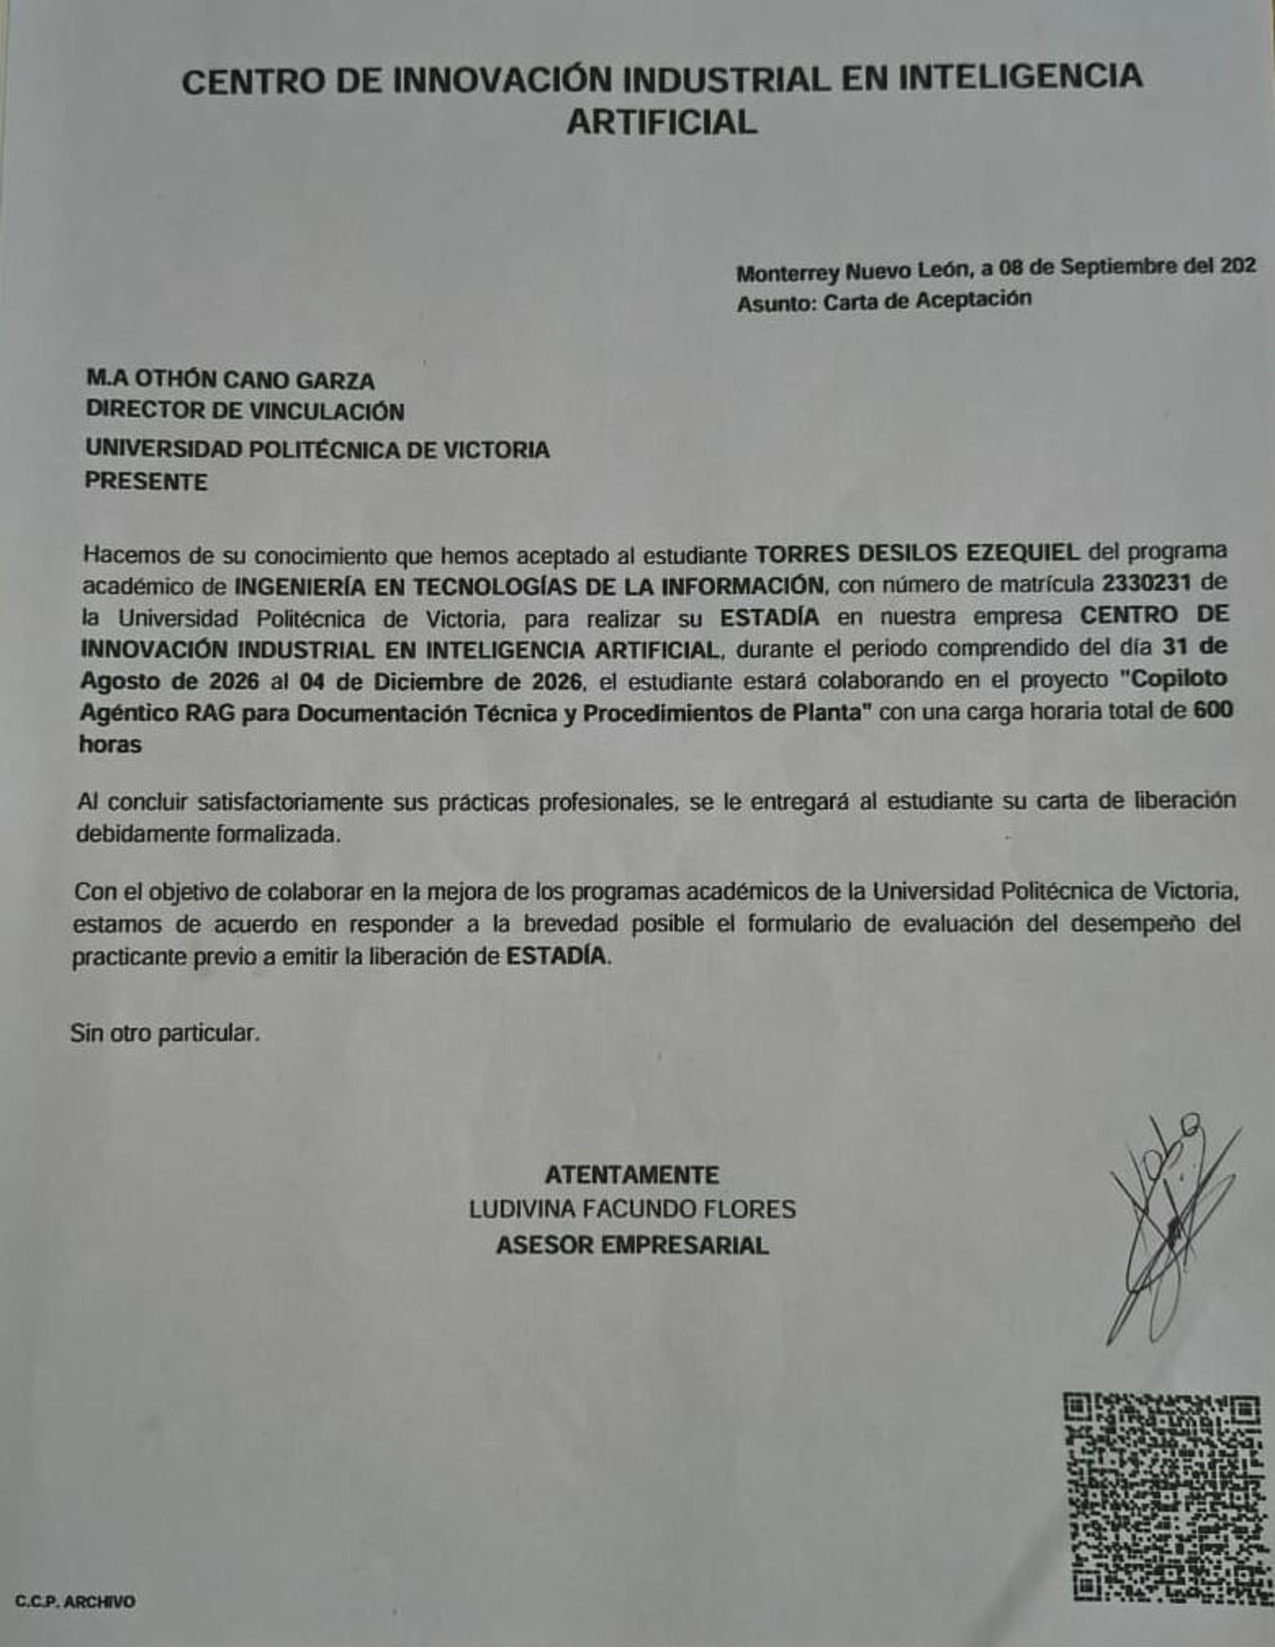
\includepdf[pages={1}]{cartas/CartaAceptacion.pdf}}{\begin{center}\vspace*{8cm}\textbf{CARTA DE ACEPTACIÓN}\\[1cm]\textit{Pendiente de integrar el PDF oficial firmado.}\end{center}}

% Pagina 3: Digitalización de la carta de liberación (sustituir por una original en el empastado)
\clearpage
\thispagestyle{fancy}
\IfFileExists{cartas/CartaLiberacion.pdf}{\includepdf[pages={1}]{cartas/CartaLiberacion.pdf}}{\begin{center}\vspace*{8cm}\textbf{CONSTANCIA DE DERECHOS / CARTA DE LIBERACIÓN}\\[1cm]\textit{Pendiente de integrar el PDF oficial firmado.}\end{center}}

% Pagina 4: Carta de aceptación del ASESOR INSTITUCIONAL(sustituir por una original en el empastado)
\clearpage
\ULCornerWallPaper{1}{Membrete2020.pdf}
\thispagestyle{empty}

\vspace*{1.5cm}
\large

\begin{center}
\textbf{CARTA DE ACEPTACIÓN DEL DOCUMENTO PARA SU IMPRESIÓN}\\[\separacionLarga]
\end{center}

\begin{flushright}
Cd. Victoria, Tamaulipas a \fechacarta \\[\separacionLarga]
\end{flushright}

\parindent=0mm

\nalumno \\
PRESENTE \\[\separacionCorta]

Le comunico que  el Programa Académico de \ncarrera\ \ le ha otorgado la autorización para la impresión de su Tesina de Estadía Práctica cuyo título es: \\[\separacionCorta]

\begin{center}
\textbf{\nproyecto} \\[\separacionLarga]
\end{center}

\begin{center}	
\begin{tabular}{ccc}
\centering
& ATENTAMENTE & \\ 
& & \\
& & \\
& & \\ \hline
& \nasesorinstitucional & \\
& ASESOR INSTITUCIONAL & \\
\end{tabular}
\end{center} 
\vspace{2cm}
c.c.p Director de programa académico


%-----------------------------------------------------------------------------------------------------------------

% Pagina 0: Rubrica de evaluación
\clearpage
\ClearWallPaper
\thispagestyle{empty}
\newgeometry{left=1.5cm,top=1.0cm,right=1.5cm,bottom=2.0cm}             
\begin{landscape}

%\afterpage{\restoregeometry}


\begin{tabular}{p{3cm}p{16cm}p{3cm}}
\multirow{4}{*}{
\includegraphics[width=3.0cm]{UTYP.png}} &  & \multirow{4}{*}{
\includegraphics[width=3.0cm]{LogoUPV_2019.png}} \\
   & \multicolumn{1}{c}{\textbf{EVALUACIÓN DE ESTADÍA}} &  \\ %\cline{2-2}
& \multicolumn{1}{c}{\textbf{Rúbrica para evaluación de la presentación y el reporte de estadía}} & \\ 
& & \\ 
\end{tabular}

\normalsize
\begin{tabular}{p{13cm}R{10cm}}
\multicolumn{1}{l}{Nombre del alumno: \underline{\textbf{\iemph{\nalumno}}}}  & 
Calificación final: \underline{\hspace{3cm}}    \\ %\cline{2-2}
\multicolumn{2}{c}{Periodo: \underline{\textbf{\iemph{\ncuatrimestre}}}}    \\ %\cline{2-2}
& \\
\end{tabular}

\scriptsize 
\begin{center}
%\resizebox{\linewidth}{!}{%
\begin{tabular}{C{2.0cm}|C{2.0cm}|C{4.0cm}|C{4.0cm}|C{4.0cm}|C{4.0cm}}
\hline
\multirow{2}{*}{Ponderación} & Aspecto a  & Competente & Independiente & Básico Avanzado & No Competente \\
 & Evaluar & 10 & 9 & 8 & 5 \\ 
\hline
40 & Resultados y Actividades & Estrechamente relacionados al perfil de
egreso de su programa académico & Parcialmente relacionados al perfil de
egreso de su programa académico & Escasamente relacionados al perfil de egreso de su programa académico & Escasamente relacionados al perfil de egreso de su programa académico \\  \hline

30 & Exposición de las actividades de la estadía  & Detalladas y sustentadas con respecto a los resultados que se obtuvieron & Detalladas y sustentadas parcialmente con respecto a los resultados que se obtuvieron & Detalladas parcialmente con respecto a los resultados que se obtuvieron & Detalladas escazamente con respecto a los resultados que se obtuvieron \\  \hline 

10 & Material visual Lenguaje
verbal & Uso el lenguaje y la terminología
apropiadas; El material visual está organizado,
adecuado y suficiente
 & 
Uso el lenguaje y la terminología apropiadas
El material visual está parcialmente
organizado y es suficiente
& 
Uso el lenguaje y la terminología son parcialmente apropiadas; El material visual está parcialmente
organizado y es suficiente
 & 
Uso el lenguaje y terminología es inapropiado; El material visual no está organizado y es insuficiente
 \\  \hline
10 & Exposición en Idioma Inglés &

Pronunciation is clear so language is easily understood (2.5) Uses fluent connected speech, occasionally disrupted by search for correct form of expression (2.5) Uses topic related vocabulary without problems (2.5) Responds to questions using varied and descriptive vocabulary and language structures (2.5) & 

Pronunciation is understandable, but there are slight errors (2.25)
Speech is connected but frequently disrupted by search for correct form of
expression (2.25) Uses some topic related vocabulary sufficient to communicate ideas (2.25) Responds to questions using simple but accurate vocabulary and language structures (2.25 & 

Pronunciation is understandable most of the time, marked native accent and many errors
(2) Speaks with simple sentences, sometimes not connected, but is understood (2) Uses basic vocabulary to communicate ideas
(2) Partly responds to simple questions, with limited vocabulary and language structures (2)  &

Pronunciation makes language very difficult to understand (1) Uses one-word/two-word utterances (1) Unable to communicate ideas due to lack of vocabulary (1) Uses isolated words or sentence fragments to respond to questions (1) 
\\  \hline

5 & Respuesta a los cuestionamientos de los evaluadores & 
Clara y satisfactoria & 
Clara y parcialmente satisfactoria & 
Clara e insuficiente & 
Confusa e insuficiente 
\\  \hline
5 & Autorización de tesina en tiempo y forma & 
Presenta en tiempo y forma  & 
Presenta en tiempo y forma con la mayoría de requerimientos solicitados & 
Presenta en tiempo y con algunas limitantes  de los requerimientos solicitados. &
Presenta fuera de tiempo y con los mínimos requerimientos solicitados.
 \\  \hline

\end{tabular}
%}
\end{center}

\normalsize


\begin{center}
\begin{tabular}{ccc}
& & \\
& & \\
\underline{\hspace{7cm}}& \underline{\hspace{7cm}} & \underline{\hspace{7cm}} \\
\nasesorinstitucional & \nevalador & \\
ASESOR INSTITUCIONAL & EVALUADOR & EVALUADOR INGLÉS \\
\end{tabular}
\end{center}

\end{landscape} 
\restoregeometry


%-----------------------------------------------------------------------------------------------------------------
% Pagina 5: Registro de Evaluación de Estadía
\clearpage
\pagestyle{empty}
\ULCornerWallPaper{1}{Membrete2020.pdf}

\vspace*{0.5cm}



\large
\begin{center}
\textbf{REGISTRO DE EVALUACION DE EXPOSICIÓN DE ESTADÍA}
\\[\separacionLarga]
\end{center}


Siendo las 0:00 hrs del día 0 de Mes de 2026, \elola\ \   
alumn\OA\ \ \textbf{\nalumno}, del programa académico \textbf{\ncarrera}, con matricula \textbf{\matricula}, presentó la exposición de la estadía realizada durante el cuatrimestre \textbf{\ncuatrimestre}, en \textbf{\organismoreceptor}, con el proyecto titulado \textbf{\nproyecto}.\\

Una vez concluido el proceso de evaluación, y con base a la rúbrica establecida para éste propósito, se determina que la calificación de la estadía es \underline{\hspace{2cm}}. %\hrulefill.

\begin{center}
\begin{tabular}{ccc}
& & \\
& & \\
& & \\
& \underline{\hspace{8cm}}& \\
& \nasesorinstitucional & \\
& ASESOR INSTITUCIONAL & \\
& & \\
& & \\
& & \\
& \underline{\hspace{8cm}}& \\
& \nevalador & \\
& EVALUADOR & \\
& & \\
& & \\
& & \\
& \underline{\hspace{8cm}}& \\
& & \\
& EVALUADOR DE INGLÉS & \\
\end{tabular}
\end{center}

\normalsize

%-----------------------------------------------------------------------------------------------------------------
% PAGINA 4 - AGRADECIMIENTOS
\clearpage
\ClearWallPaper
\pagestyle{fancy}
\section*{\centering Agradecimientos}
\addcontentsline{toc}{section}{Agradecimientos}
% Sección reservada; contenido pendiente.


%-----------------------------------------------------------------------------------------------------------------
% PAGINA 5 - RESUMEN EN ESPAÑOL

\clearpage
\section*{\centering Resumen}
\addcontentsline{toc}{section}{Resumen}
% Sección reservada; contenido pendiente.


%-----------------------------------------------------------------------------------------------------------------
% PAGINA 6 - RESUMEN EN INGLES

\clearpage
\section*{\centering Summary}
\addcontentsline{toc}{section}{Summary}
% Sección reservada; contenido pendiente.


%-----------------------------------------------------------------------------------------------------------------
% PAGINA 7 - INDICE

\clearpage
\addcontentsline{toc}{section}{Índice}
\renewcommand\contentsname{Índice}
\tableofcontents

\clearpage
\addcontentsline{toc}{section}{Índice de figuras}
\renewcommand\listfigurename{Índice de figuras}

\listoffigures

\clearpage
\addcontentsline{toc}{section}{Índice de cuadros}
\renewcommand\listtablename{Índice de cuadros}
\listoftables

%\clearpage
%\addcontentsline{toc}{section}{Índice de algoritmos}
%\renewcommand\listalgorithmname{Índice de algoritmos}
%\listofalgorithms

%-----------------------------------------------------------------------------------------------------------------
% CAPITULOS


\clearpage
\pagenumbering{arabic}
\setcounter{page}{1}
\section{Introducción}

En las organizaciones que desarrollan soluciones tecnológicas para la industria, la documentación representa una parte importante del conocimiento operativo. Manuales, instructivos, procedimientos, políticas, reportes y especificaciones contienen información que debe consultarse para realizar actividades de manera uniforme. Sin embargo, la existencia de los documentos no garantiza que la información pueda localizarse con rapidez. Cuando los archivos se encuentran distribuidos en diferentes carpetas, tienen formatos distintos o utilizan una terminología que no coincide con la pregunta del usuario, la consulta puede convertirse en una actividad lenta y dependiente de la experiencia de una persona.

En un entorno de innovación industrial, esta situación adquiere una importancia adicional. Las soluciones se diseñan, prueban y modifican con frecuencia, por lo que la información técnica puede cambiar durante el ciclo de vida de un proyecto. Un integrante que necesita conocer un procedimiento no solo requiere una respuesta rápida; también necesita saber de qué documento provino la información, qué página o sección la contiene y si el material consultado corresponde a la versión vigente. La trazabilidad permite revisar la respuesta, corregir errores y evitar que una recomendación generada automáticamente se interprete como una instrucción oficial sin respaldo.

La inteligencia artificial (IA) generativa ofrece una forma natural de interactuar con la información mediante preguntas en lenguaje cotidiano. Un modelo de lenguaje puede interpretar la intención del usuario, resumir un texto y organizar una explicación. No obstante, si se consulta el modelo sin información específica de la organización, puede responder con conocimiento general, mezclar conceptos o producir una afirmación que parece correcta pero no está sustentada por los procedimientos internos. En consecuencia, la aplicación de inteligencia artificial a la documentación técnica requiere una arquitectura que combine generación, recuperación de información y control de fuentes \citep{lewis2020rag,gao2023rag}.

El presente proyecto propone la base de un copiloto agéntico basado en recuperación aumentada por generación (RAG, por sus siglas en inglés) para documentación técnica y procedimientos de planta. La solución integra una interfaz web, una interfaz de programación de aplicaciones (API, por sus siglas en inglés) propia y un flujo de inteligencia artificial. La interfaz permite que una persona escriba una pregunta y observe la conversación. El backend recibe la solicitud, valida sus datos y se comunica con el proveedor externo de IA. La arquitectura también contempla un recuperador semántico que buscará fragmentos relevantes en una colección documental, construirá el contexto de la consulta y devolverá una respuesta acompañada de fuentes. Este enfoque se fundamenta en la combinación de recuperación y generación descrita en la literatura especializada \citep{lewis2020rag,gao2023rag}.

En esta etapa se desarrolla la base necesaria para que los componentes puedan integrarse sin depender de una sola tecnología de interfaz o de un único proveedor de modelos. El frontend se implementa con HTML (HyperText Markup Language, lenguaje de marcado de hipertexto), CSS (Cascading Style Sheets, hojas de estilo en cascada) y JavaScript, mientras que el backend se construye con Python y FastAPI. La comunicación se realiza mediante HTTP (HyperText Transfer Protocol, protocolo de transferencia de hipertexto) y JSON (JavaScript Object Notation, notación de objetos de JavaScript). FastAPI proporciona validación de solicitudes y documentación interactiva de la API mediante OpenAPI \citep{fastapiDocs}. El proveedor de IA se consume desde el servidor para evitar que la clave de acceso quede expuesta en el navegador. La recuperación documental se define como una responsabilidad separada, de manera que los documentos, embeddings y metadatos puedan conectarse posteriormente al agente.

El proyecto se desarrolla en colaboración con el Centro de Innovación Industrial en Inteligencia Artificial, CII.IA, ubicado en Monterrey, Nuevo León, México. La organización comunica una orientación hacia la aplicación y el escalamiento de soluciones de inteligencia artificial para la industria, contexto que sustenta la pertinencia de una herramienta de consulta documental \citep{ciiia2026,ciiia2026b}. El resultado esperado no es únicamente una pantalla de conversación, sino una base técnica y documental para una herramienta que pueda crecer con el corpus institucional. A partir de esta base será posible incorporar criterios de similitud, reglas para detectar falta de contexto, fuentes consultables y pruebas que comparen las respuestas del agente con los documentos originales.

\subsection{Antecedentes}

La consulta de información ha pasado por diferentes etapas. En un primer momento, el usuario debía conocer la ubicación física o digital del documento y revisarlo manualmente. Posteriormente, los sistemas de archivos y las herramientas de búsqueda permitieron localizar palabras dentro de varios documentos. Aunque estos mecanismos reducen el tiempo de consulta, dependen de que el usuario utilice exactamente las mismas palabras que aparecen en el material. Una persona puede preguntar ``¿qué se debe hacer antes de iniciar el equipo?'' aunque el documento utilice una expresión como ``verificación previa a la puesta en operación''.

La búsqueda semántica intenta resolver esta diferencia al comparar el significado aproximado de la pregunta con el significado de los fragmentos documentales. Para ello, cada fragmento se transforma en un embedding y se almacena con información que permite rastrear su origen. El modelo generativo interviene después de la recuperación y utiliza el contexto seleccionado para elaborar una respuesta comprensible. Esta combinación se conoce como recuperación aumentada por generación.

El crecimiento de los modelos de lenguaje ha impulsado interfaces conversacionales para consultar bases de conocimiento. Sin embargo, un chatbot que no tenga conexión con el corpus de la organización no es suficiente para una consulta técnica controlada. Puede utilizar información que no está vigente, responder de forma general o no distinguir entre una recomendación y un procedimiento autorizado. La propuesta de este proyecto parte de esta diferencia: la conversación es el medio de interacción, pero los documentos deben ser la base de la respuesta.

\subsubsection{Antecedentes tecnológicos}

La arquitectura se apoya en tecnologías web y de servicios. HTML organiza los elementos de la pantalla, CSS define la distribución visual y JavaScript controla eventos, solicitudes y actualización del contenido. FastAPI permite declarar rutas, modelos de datos y validaciones para el servicio. Uvicorn ejecuta la aplicación ASGI (Asynchronous Server Gateway Interface, interfaz de puerta de enlace de servidor asíncrono) durante el desarrollo. La comunicación entre ambos extremos se realiza con solicitudes HTTP y objetos JSON.

Para la parte de inteligencia artificial se considera el consumo de un modelo externo mediante HTTPS (HyperText Transfer Protocol Secure, protocolo seguro de transferencia de hipertexto). El agente puede utilizar componentes de LangChain para preparar prompts y conectar un modelo con un recuperador, y LangGraph puede representar las decisiones del flujo mediante estados. PostgreSQL con capacidades vectoriales se contempla para almacenar embeddings y metadatos. Estas tecnologías se integran por capas, evitando que la lógica de recuperación quede mezclada con la presentación de la interfaz.

La seguridad básica también forma parte de los antecedentes del proyecto. Las claves de API deben existir únicamente en el entorno del backend, normalmente mediante un archivo `.env` que no se publica. El servidor debe validar la entrada antes de enviarla al proveedor y el frontend no debe conocer las credenciales. CORS (Cross-Origin Resource Sharing, intercambio de recursos de origen cruzado) se utiliza para controlar la comunicación entre el origen del frontend y el origen del backend durante el desarrollo.

\subsubsection{Antecedentes de la empresa}

El Centro de Innovación Industrial en Inteligencia Artificial, CII.IA, es una organización ubicada en Monterrey, Nuevo León, México, orientada a la aplicación de inteligencia artificial en contextos empresariales e industriales. Su trabajo relaciona la identificación de necesidades con el diseño, prototipado, validación y posible escalamiento de soluciones tecnológicas. Este contexto requiere que el conocimiento generado durante los proyectos pueda organizarse y consultarse de forma eficiente.

La creación de un copiloto documental se relaciona con esa necesidad porque convierte procedimientos y documentos técnicos en una fuente consultable mediante lenguaje natural. La herramienta no pretende reemplazar la responsabilidad de quien toma decisiones ni sustituir la validación de un experto. Su función inicial es apoyar la localización, comprensión y trazabilidad de la información, manteniendo visible el origen de los fragmentos utilizados.

El proyecto también es congruente con un ambiente de innovación porque utiliza una arquitectura que puede evolucionar. En una primera versión se valida la comunicación entre frontend, backend y modelo. En etapas posteriores se pueden incorporar nuevos documentos, actualizar embeddings, agregar reglas de evaluación y adaptar el flujo a otras áreas o tipos de procedimiento.

\subsection{Planteamiento del problema}

El problema se presenta cuando una persona necesita consultar una indicación técnica y no tiene un mecanismo uniforme para localizarla. La información puede estar dispersa en documentos distintos, contener versiones previas o emplear términos diferentes a los de la pregunta. La búsqueda manual consume tiempo y puede producir interpretaciones diferentes entre usuarios. Una búsqueda literal no siempre identifica fragmentos que expresan la misma idea con otras palabras.

La incorporación directa de un modelo de lenguaje tampoco resuelve por sí sola el problema. Aunque el modelo puede redactar una respuesta clara, no existe garantía de que utilice la documentación interna, de que conozca la versión vigente o de que pueda señalar la página donde obtuvo la información. En un procedimiento de planta, esta falta de trazabilidad representa una limitación importante.

Por lo tanto, el problema de investigación y desarrollo se formula de la siguiente manera: ¿cómo diseñar e implementar la base de un copiloto web que facilite la consulta de documentación técnica mediante inteligencia artificial, se comunique de manera segura con un backend, utilice un flujo preparado para recuperación semántica y devuelva respuestas con fuentes verificables?

El problema puede dividirse en cuatro aspectos. El primero es la interacción: se necesita una interfaz sencilla para escribir preguntas y leer respuestas. El segundo es la integración: se necesita una API que valide y coordine la solicitud. El tercero es el conocimiento: se necesita un corpus con fragmentos, embeddings y metadatos. El cuarto es el control: se necesitan reglas para indicar falta de información, manejar errores y evitar que una respuesta generada se presente como un procedimiento oficial sin evidencia.

\subsection{Objetivo general}

Desarrollar la base funcional de un copiloto agéntico RAG para consultar documentación técnica y procedimientos de planta, integrando una interfaz web, una API con FastAPI y un modelo externo de inteligencia artificial, con una arquitectura preparada para recuperar fragmentos documentales, conservar sus metadatos y presentar fuentes verificables.

\subsection{Objetivos específicos}

\begin{enumerate}
    \item Analizar la necesidad de consulta documental y delimitar el alcance funcional de la primera versión.
    \item Identificar los actores, entradas, salidas y restricciones que intervienen en una consulta al copiloto.
    \item Diseñar una interfaz web que permita escribir preguntas, enviar solicitudes y visualizar respuestas.
    \item Implementar una API con FastAPI para recibir, validar y responder solicitudes de conversación.
    \item Configurar CORS y el intercambio de datos en formato JSON entre el frontend y el backend.
    \item Integrar un proveedor externo de inteligencia artificial mediante variables de entorno protegidas.
    \item Definir el flujo de validación, recuperación, construcción de contexto y generación de respuestas.
    \item Establecer un contrato para fragmentos documentales que incluya identificador, contenido, archivo, página, sección y puntuación.
    \item Aplicar reglas para que el agente indique cuando no cuenta con información suficiente y evite inventar procedimientos.
    \item Preparar pruebas de comunicación entre frontend, backend, recuperador y modelo externo.
    \item Documentar la arquitectura, las decisiones técnicas, las limitaciones y las actividades pendientes.
\end{enumerate}

\subsection{Justificación}

Un copiloto para documentación técnica puede reducir el tiempo que se dedica a localizar información y facilitar el acceso al conocimiento organizacional. En lugar de depender de que el usuario recuerde el nombre de un archivo o revise manualmente varias carpetas, la interfaz permite formular una pregunta de manera natural. El resultado puede resumir el contenido y dirigir al usuario hacia el documento que debe revisar.

La propuesta es especialmente útil cuando la documentación contiene procedimientos repetitivos, definiciones técnicas o instrucciones que deben consultarse con frecuencia. La recuperación semántica puede identificar fragmentos relacionados aunque la redacción de la pregunta no coincida literalmente con la redacción del documento. La inclusión de metadatos permite que la respuesta sea revisable y que un responsable confirme la información antes de utilizarla en una actividad crítica.

Desde el punto de vista de desarrollo, el proyecto permite integrar conocimientos de frontend, backend, APIs, bases de datos, procesamiento de lenguaje natural y evaluación de inteligencia artificial. La separación de componentes facilita que el diseño visual pueda cambiar sin alterar el servicio, que el proveedor de IA pueda sustituirse y que la fuente documental pueda actualizarse sin reconstruir toda la aplicación.

La propuesta también es justificable por su enfoque de control. No se plantea un chatbot abierto que responda cualquier tema, sino un copiloto limitado a un dominio documental. Cuando el contexto no sea suficiente, el sistema debe comunicar esa condición. Esta decisión es importante porque una respuesta negativa y verificable es preferible a una respuesta extensa sin respaldo.

\subsection{Alcances y limitaciones}

Para delimitar con claridad la primera versión del proyecto, los alcances y las limitaciones se presentan de forma independiente.

\subsubsection{Alcances}

\begin{itemize}
    \item Analizar la necesidad de consulta de documentación técnica y definir el flujo general del copiloto.
    \item Mantener una interfaz web para que el usuario escriba preguntas, envíe solicitudes y consulte las respuestas recibidas.
    \item Implementar una API con FastAPI para validar la solicitud de conversación y devolver una respuesta en formato JSON.
    \item Configurar la comunicación entre frontend y backend mediante CORS, conservando la clave del proveedor de IA únicamente en el servidor.
    \item Integrar un modelo externo de inteligencia artificial mediante variables de entorno y un contrato de respuesta controlado.
    \item Definir la arquitectura RAG, incluyendo la consulta, la recuperación de contexto, la construcción del prompt y la generación de la respuesta.
    \item Especificar los metadatos mínimos de cada fragmento: \texttt{chunk\_id}, contenido, archivo de origen, página, sección y puntuación.
    \item Preparar la integración con la colección de documentos técnicos, sus embeddings, el almacenamiento vectorial y la búsqueda semántica entregada por el Integrante 1.
    \item Incluir fuentes y estados de respuesta para que el resultado pueda revisarse y distinguirse de una respuesta sin evidencia.
    \item Documentar la tabla comparativa, las decisiones de diseño, las pruebas de comunicación y las actividades pendientes.
\end{itemize}

\subsubsection{Limitaciones}

\begin{itemize}
    \item La respuesta depende de la disponibilidad, cuota, autenticación y modelo seleccionado en el proveedor externo de inteligencia artificial.
    \item La calidad de la respuesta depende de que los documentos estén completos, vigentes, correctamente fragmentados y acompañados de sus metadatos.
    \item La búsqueda semántica no garantiza por sí sola que un fragmento contenga toda la respuesta; por ello se requiere un umbral de similitud y validación del contexto.
    \item La colección documental, la carga de embeddings y el endpoint de búsqueda deben validarse con los datos autorizados y entregados por el Integrante 1.
    \item El sistema no sustituye la revisión de una persona responsable cuando la consulta se relaciona con seguridad, calidad, operación o una decisión crítica.
    \item La primera versión se limita al dominio de documentación técnica y procedimientos de planta; no se considera un chatbot de propósito general.
    \item El cambio de proveedor, la actualización del corpus y el despliegue en producción requieren configuraciones y pruebas adicionales.
\end{itemize}

\subsection{Organización del documento de tesina}

El Capítulo 1 presenta la introducción, los antecedentes generales, los antecedentes tecnológicos y de la empresa, el planteamiento del problema, los objetivos, la justificación, los alcances y las limitaciones. El Capítulo 2 desarrolla los antecedentes teóricos, los conceptos de inteligencia artificial generativa, RAG, embeddings, agentes, APIs, bases vectoriales y evaluación, además de los temas tentativos del marco teórico.

El Capítulo 3 presenta el estado del arte y los trabajos relacionados con la consulta de información, además de la tabla comparativa de alternativas. El Capítulo 4 conserva la sección destinada al desarrollo del proyecto. El Capítulo 5 se reserva para describir el sistema propuesto y su arquitectura. El Capítulo 6 contiene la estructura para documentar la implementación y las pruebas. El Capítulo 7 conserva el espacio para conclusiones y trabajo futuro. Las secciones de agradecimientos, resumen y summary se dejan vacías en esta versión para completarlas posteriormente.


\clearpage
\section{Marco teórico}

\subsection{Antecedentes teóricos}

El marco teórico de este proyecto reúne los conceptos que permiten relacionar una interfaz conversacional con una fuente de documentación controlada. La solución propuesta no se limita a consumir un modelo de lenguaje; requiere una cadena de procesamiento en la que la pregunta se valide, el conocimiento relevante se recupere, el contexto se entregue al modelo y la respuesta se devuelva con información suficiente para revisarla.

La arquitectura se analiza desde cuatro perspectivas. La primera es la inteligencia artificial generativa, que produce una respuesta a partir de una instrucción. La segunda es la recuperación semántica, que localiza fragmentos relacionados con la pregunta. La tercera es la ingeniería de software, que organiza el frontend, backend y contratos de comunicación. La cuarta es la confiabilidad, que incluye fuentes, guardrails, manejo de errores y evaluación.

Los antecedentes teóricos se relacionan directamente con las etapas del sistema: preparación del conocimiento, recepción de la pregunta, recuperación de información, generación de la respuesta y validación del resultado. La siguiente tabla resume esa relación y permite identificar qué aporta cada concepto al diseño del copiloto.

\renewcommand{\arraystretch}{1.25}
\begin{longtable}{p{3.4cm}p{5.0cm}p{5.5cm}}
\caption{Antecedentes teóricos y relación con el proyecto.}\label{tab:antecedentes-teoricos}\\\toprule
\textbf{Antecedente teórico} & \textbf{Concepto principal} & \textbf{Relación con el copiloto documental}\\\midrule
\endfirsthead
\toprule
\textbf{Antecedente teórico} & \textbf{Concepto principal} & \textbf{Relación con el copiloto documental}\\\midrule
\endhead
\bottomrule
\endfoot
Inteligencia artificial generativa & Modelos capaces de interpretar instrucciones y producir texto. & Permite redactar una respuesta comprensible a partir de la pregunta y del contexto documental recuperado.\\
Recuperación aumentada por generación & Integración de búsqueda de información y generación de lenguaje. & Evita que la respuesta dependa únicamente del conocimiento general del modelo y permite fundamentarla con fragmentos.\\
Embeddings y similitud semántica & Representación vectorial de textos y comparación por cercanía. & Permite localizar fragmentos relacionados aunque la pregunta utilice palabras diferentes a las del documento.\\
Metadatos y trazabilidad & Datos que describen el origen, ubicación y versión de un fragmento. & Hace posible mostrar el archivo, página, sección, identificador y puntuación de los resultados.\\
Agentes y toma de decisiones & Flujo compuesto por estados, condiciones y acciones. & Organiza la validación, la recuperación, la generación, el rechazo por falta de contexto y el escalamiento.\\
Servicios web y contratos de datos & Comunicación entre componentes mediante solicitudes y respuestas estructuradas. & Define cómo el frontend envía la pregunta y cómo recibe el texto, las fuentes y el estado de la operación.\\
Evaluación y confiabilidad & Medición de relevancia, fidelidad, claridad, errores y límites de uso. & Permite determinar si las respuestas son útiles, verificables y adecuadas para el dominio técnico.\\
\end{longtable}

El cuadro muestra que la solución no depende de un único concepto. La generación aporta la capacidad de redactar, pero la recuperación aporta el conocimiento específico; los metadatos permiten verificarlo y la evaluación establece si el resultado es aceptable. Esta relación será utilizada como guía para documentar el desarrollo y las pruebas posteriores.

\subsection{Inteligencia artificial generativa y modelos de lenguaje}

La inteligencia artificial generativa comprende métodos capaces de crear contenido a partir de patrones aprendidos. En el caso de los modelos de lenguaje, el contenido se produce mediante la predicción y organización de unidades de texto. Estos modelos pueden interpretar preguntas, seguir instrucciones, resumir información y producir respuestas con diferentes estilos.

Una característica importante es que el modelo no consulta automáticamente los procedimientos internos de una organización. Su conocimiento depende de los datos con los que fue entrenado y de la información que se le proporcione durante la solicitud. Por esta razón, una aplicación técnica debe separar la capacidad lingüística del modelo de la autoridad documental de la organización.

El prompt cumple la función de establecer el contexto y las reglas. Puede indicar el papel del agente, el formato de la respuesta, la obligación de utilizar únicamente los fragmentos proporcionados y la acción que debe realizarse cuando el contexto no sea suficiente. Sin embargo, un prompt por sí solo no garantiza que la respuesta sea correcta; debe combinarse con recuperación, metadatos y evaluación.

\subsection{Recuperación aumentada por generación}

La recuperación aumentada por generación, conocida como RAG, es un enfoque que combina una etapa de recuperación de información con una etapa de generación de texto. La pregunta se utiliza para localizar fragmentos relacionados y esos fragmentos se incorporan a la solicitud que recibe el modelo. La respuesta se construye entonces con base en el contexto recuperado, en lugar de depender únicamente del conocimiento general del modelo \citep{lewis2020rag,gao2023rag}.

El flujo RAG puede dividirse en una fase de preparación y una fase de consulta. En la preparación se recopilan los documentos, se extrae su texto, se dividen en fragmentos y se calcula un embedding para cada fragmento. En la consulta se calcula el embedding de la pregunta, se comparan vectores, se seleccionan los resultados con mayor similitud y se prepara el prompt. Esta separación permite actualizar el corpus sin reentrenar el modelo generativo.

La calidad de un sistema RAG depende de más factores que el modelo. Un fragmento demasiado grande puede contener información irrelevante; uno demasiado pequeño puede perder el contexto necesario. La selección de \texttt{top\_k} también influye: pocos fragmentos pueden omitir información, mientras que demasiados pueden hacer que el prompt sea extenso o confuso. Por lo tanto, la configuración debe probarse con preguntas representativas del dominio.

\subsection{Fragmentación de documentos}

La fragmentación, o división en chunks, transforma un documento extenso en unidades que pueden indexarse y recuperarse. La estrategia debe conservar la relación entre el texto y su ubicación original. Un fragmento puede corresponder a un párrafo, una sección, una lista o una combinación controlada de varios elementos.

El tamaño del fragmento debe equilibrar detalle y contexto. El solapamiento entre fragmentos puede evitar que una idea quede dividida entre dos unidades sin relación, pero también aumenta el número de vectores almacenados. La estrategia seleccionada debe considerar el tipo de documento, la longitud de los procedimientos, los títulos y la presencia de tablas o listas.

Los metadatos son tan importantes como el texto. Para este proyecto se requiere conservar al menos el identificador del fragmento, el contenido, el archivo de origen, el número de página, la sección y la puntuación obtenida en la búsqueda. También pueden agregarse versión, fecha de actualización, área responsable y tipo de documento.

\subsection{Embeddings y búsqueda semántica}

Un embedding representa un texto como un vector numérico dentro de un espacio en el que los textos con significado parecido tienden a estar próximos. La pregunta del usuario y los fragmentos documentales deben transformarse utilizando un proceso compatible para que la comparación sea significativa.

La similitud puede calcularse mediante distancia coseno, producto punto u otra métrica soportada por el motor vectorial. La función de búsqueda recibe una pregunta y el valor de \texttt{top\_k}, y devuelve los fragmentos ordenados por su puntuación. El backend debe conservar esa puntuación para que el sistema pueda establecer un umbral de suficiencia y explicar por qué seleccionó un resultado.

La búsqueda semántica no debe interpretarse como una prueba absoluta de verdad. Un fragmento puede ser similar a la pregunta y, aun así, no contener la respuesta completa. Por ello, el agente debe revisar la suficiencia del contexto, utilizar instrucciones de no invención y permitir que el usuario consulte la fuente original.

\subsection{Bases de datos vectoriales y metadatos}

Una base de datos vectorial almacena embeddings junto con los datos que describen a cada registro. PostgreSQL con una extensión vectorial es una alternativa para mantener en un mismo sistema el contenido, los metadatos y el vector. Esto permite consultar fragmentos por similitud y filtrar por documento, sección, versión o área.

La tabla documental debe diseñarse para que los cambios puedan rastrearse. Un registro puede tener un identificador único, texto del fragmento, vector, archivo de origen, página, sección, fecha de carga y versión. Si un documento deja de estar vigente, se debe poder marcarlo o retirarlo sin perder el historial necesario para comprender una prueba anterior.

La carga de embeddings y la función de búsqueda semántica pertenecen a la integración documental. En este proyecto se deja establecido el contrato que necesita el agente para consumir esa función, pero los datos finales deben provenir del corpus autorizado y del trabajo correspondiente del Integrante 1.

\subsection{Modelos externos de inteligencia artificial}

El modelo externo se consume mediante una solicitud HTTPS. La aplicación envía un prompt compuesto por instrucciones, pregunta y contexto recuperado, y recibe una respuesta generada. La documentación de Gemini describe modelos que reciben contenido y devuelven candidatos de respuesta a través de una API generativa \citep{googleGeminiApi}. Un proveedor equivalente puede utilizarse siempre que respete el contrato del backend.

La integración debe contemplar errores de autenticación, modelo inexistente, límite de solicitudes, contenido rechazado, tiempos de espera y fallos de red. El backend debe transformar esos casos en estados comprensibles para el frontend, sin mostrar la clave ni datos sensibles en los mensajes.

\subsection{Agentes y orquestación de flujos}

Un agente coordina herramientas y pasos para resolver una pregunta. En el flujo propuesto, el agente recibe la consulta, determina si pertenece al dominio, solicita los fragmentos relevantes, construye el contexto, consulta al modelo y revisa la respuesta. La salida debe incluir el texto y la evidencia utilizada.

La orquestación puede representarse como una secuencia o como un grafo de estados y transiciones. Por ejemplo, después de la búsqueda puede existir una condición que dirija el flujo hacia la generación si hay suficiente información o hacia una respuesta de incertidumbre si no la hay. En la implementación, este comportamiento puede apoyarse en bibliotecas de orquestación como LangChain y LangGraph, pero el fundamento teórico es la separación de estados, decisiones y responsabilidades \citep{langchainDocs,langgraphDocs}.

La orquestación no elimina la necesidad de un backend. El servicio web sigue funcionando como la frontera de la aplicación, controla la entrada, protege la configuración y devuelve el contrato que utiliza el frontend. La lógica del agente se ubica dentro de una capa independiente para que pueda probarse y sustituirse sin modificar la interfaz.

\subsection{Servicios web, contratos de comunicación y control de origen}

Una API REST (Representational State Transfer) expone operaciones mediante rutas HTTP. Un framework de backend como FastAPI permite definir modelos de entrada con tipos, validar solicitudes y producir documentación interactiva a partir del esquema OpenAPI \citep{fastapiDocs}. El servidor de aplicación ejecuta estas rutas durante el desarrollo y el despliegue.

La ruta principal del proyecto es \texttt{POST /chat}. La solicitud recibe un objeto JSON con la propiedad \texttt{message}. El backend valida que la propiedad exista y que su contenido sea utilizable. Después procesa la pregunta y devuelve un objeto que puede incluir \texttt{reply}, \texttt{sources} y \texttt{status}.

El navegador aplica la política de mismo origen. Si el frontend y el backend se ejecutan en puertos diferentes, la solicitud puede ser bloqueada aunque ambos procesos estén activos. CORS permite declarar los orígenes autorizados, métodos y encabezados que pueden utilizarse. En producción, la lista debe ser más restrictiva que durante el desarrollo.

\subsection{Variables de entorno y protección de credenciales}

Una variable de entorno permite configurar una aplicación sin escribir el secreto directamente en el código. La clave del proveedor y el nombre del modelo deben leerse en el backend. El archivo `.env` debe agregarse al archivo de exclusión de Git y nunca debe enviarse al repositorio.

El frontend no debe intentar comunicarse directamente con el proveedor de IA porque eso expondría la clave en el navegador. La API propia actúa como intermediaria, aplica validaciones, registra estados y puede añadir guardrails antes de enviar la solicitud.

\subsection{Guardrails, fuentes y evaluación}

Los guardrails son reglas que limitan o revisan el comportamiento del agente. En el proyecto deben cubrir preguntas fuera del dominio, ausencia de contexto, respuestas que no coincidan con las fuentes, errores del proveedor y solicitudes que requieran intervención humana. El agente debe preferir indicar ``no se encontró información suficiente'' antes que completar una instrucción mediante una suposición.

Las fuentes deben mostrar al menos el archivo, la página, la sección, el identificador del fragmento y la puntuación. Esto permite revisar la respuesta y comparar el texto generado con el material original. En una etapa posterior también se pueden incluir enlaces internos, versiones y fechas de vigencia.

La evaluación debe medir relevancia de la recuperación, exactitud de la respuesta, cobertura de las preguntas, fidelidad al contexto, claridad, latencia y comportamiento ante errores. El marco de gestión de riesgos de IA del Instituto Nacional de Estándares y Tecnología (NIST, National Institute of Standards and Technology) propone considerar confiabilidad, transparencia, seguridad y responsabilidad \citep{nistAirmf}.

\subsection{Temas tentativos para el marco teórico}

Los siguientes temas quedan propuestos para la revisión del marco teórico. Cada uno se delimita por su relación con el problema, de modo que no se presente únicamente como una lista de tecnologías utilizadas:

\begin{enumerate}
    \item \textbf{Inteligencia artificial generativa y modelos de lenguaje:} principios de generación de texto, interpretación de instrucciones, límites del conocimiento aprendido y necesidad de proporcionar contexto.
    \item \textbf{Recuperación aumentada por generación:} etapas de preparación y consulta, relación entre recuperación y generación, ventajas, riesgos y criterios de suficiencia del contexto.
    \item \textbf{Procesamiento de documentos técnicos:} extracción, limpieza, normalización y conservación de la estructura necesaria para consultar procedimientos.
    \item \textbf{Fragmentación y solapamiento:} criterios para dividir documentos, tamaño de los fragmentos, preservación del contexto y efecto del solapamiento en la recuperación.
    \item \textbf{Embeddings y métricas de similitud:} representación vectorial, comparación de textos, puntuaciones, ordenamiento de resultados y umbrales de aceptación.
    \item \textbf{Almacenamiento vectorial:} organización de vectores, contenido y metadatos; filtros por documento, versión, sección o área responsable.
    \item \textbf{Metadatos, versiones y trazabilidad documental:} identificación del fragmento, archivo de origen, página, sección, vigencia y relación entre respuesta y evidencia.
    \item \textbf{Ingeniería de prompts y construcción de contexto:} instrucciones del agente, formato de salida, delimitación del contexto, citas y respuesta ante información insuficiente.
    \item \textbf{Agentes y orquestación de flujos:} estados, decisiones, recuperación, generación, guardrails, respuesta de incertidumbre y escalamiento a una persona responsable.
    \item \textbf{Servicios web y contratos de datos:} rutas, validación, solicitudes y respuestas estructuradas para comunicar la interfaz con el backend.
    \item \textbf{Comunicación entre capas y control de origen:} intercambio de datos, JSON, CORS, autenticación básica y protección de credenciales.
    \item \textbf{Guardrails y prevención de respuestas no sustentadas:} restricciones de dominio, detección de falta de contexto, manejo de errores y prevención de alucinaciones.
    \item \textbf{Evaluación de sistemas RAG:} relevancia de recuperación, fidelidad al contexto, exactitud, claridad, cobertura, latencia y comportamiento ante fallos.
\end{enumerate}

La selección anterior mantiene el marco teórico centrado en los conceptos que explican el problema y la solución. Las bibliotecas, lenguajes y servicios específicos se documentarán posteriormente en el capítulo de desarrollo como decisiones de implementación, no como temas independientes del marco teórico.


\clearpage
\section{Estado del arte y trabajos relacionados}

La consulta de información técnica puede abordarse mediante distintas estrategias. La opción más sencilla consiste en revisar manualmente los documentos. También pueden utilizarse buscadores por palabras clave, bases de datos relacionales, chatbots conectados a un modelo de lenguaje o sistemas RAG. La diferencia principal se encuentra en la forma en que cada alternativa interpreta la pregunta, recupera la información y permite verificar la respuesta.

En una organización dedicada a la innovación, la solución debe considerar que el corpus puede crecer y cambiar. Un mecanismo útil no debe limitarse a encontrar una coincidencia de texto; debe conservar la relación entre la respuesta y el documento de origen. También debe permitir que un responsable detecte cuándo la pregunta no puede responderse con la información disponible.

\subsection{Búsqueda manual de procedimientos}

La búsqueda manual consiste en explorar carpetas, archivos y páginas hasta encontrar la instrucción requerida. Su ventaja es que la persona revisa directamente el documento y puede interpretar elementos que un sistema automático no reconoce. Además, no requiere infraestructura adicional.

Su principal desventaja es el tiempo. El usuario debe conocer la ubicación, el nombre o la estructura del archivo. Cuando existen documentos similares o versiones antiguas, aumenta la posibilidad de consultar material incorrecto. El resultado también depende de la experiencia de cada persona, por lo que el proceso no siempre es uniforme.

\subsection{Búsqueda por palabras clave}

La búsqueda por palabras clave permite localizar coincidencias dentro de varios documentos. Es fácil de implementar, tiene un costo bajo y funciona bien cuando la colección es pequeña y el usuario conoce los términos exactos. Puede complementarse con filtros por fecha, tipo de archivo o área.

La limitación es que la coincidencia literal no comprende necesariamente el significado. Una pregunta con sinónimos, abreviaturas o una estructura distinta puede no devolver el documento correcto. También puede producir demasiados resultados si una palabra aparece en muchas secciones, sin explicar cuál de ellos responde realmente a la pregunta.

\subsection{Chatbot sin recuperación documental}

Un chatbot conectado directamente a un modelo de lenguaje ofrece una interacción natural. El usuario puede preguntar sin conocer la organización de los documentos y recibe una respuesta redactada con rapidez. Esta alternativa es útil para tareas generales de explicación o generación de texto.

Para procedimientos técnicos, el chatbot sin recuperación presenta riesgos. Puede usar conocimiento externo al dominio, mezclar versiones, inventar pasos o no ser capaz de señalar la fuente. La respuesta puede ser lingüísticamente correcta y, al mismo tiempo, no corresponder al procedimiento oficial. Por esta razón, se considera una solución incompleta para el problema de este proyecto.

\subsection{Sistemas de recuperación aumentada por generación}

Los sistemas RAG agregan una etapa que busca fragmentos antes de consultar al modelo. El buscador semántico puede identificar información relacionada aunque la pregunta y el documento no utilicen exactamente las mismas palabras. El modelo recibe los fragmentos como contexto y puede generar una explicación con referencias.

Esta alternativa introduce nuevos retos. La calidad de la respuesta depende de la ingesta, la segmentación, los embeddings, el motor vectorial, el valor de \texttt{top\_k}, el prompt y la evaluación. Si el recuperador no encuentra el fragmento adecuado, el modelo puede recibir un contexto incompleto. Por ello, el sistema debe conservar las puntuaciones y establecer reglas para declarar insuficiencia.

\subsection{Copilotos documentales en entornos técnicos}

Un copiloto documental se diferencia de un chatbot general porque trabaja con un dominio, un corpus y una responsabilidad definida. Puede responder preguntas frecuentes, resumir instrucciones y dirigir al usuario hacia la fuente. La decisión final permanece en la persona responsable, especialmente cuando la información afecta seguridad, calidad, operación o cumplimiento.

El diseño propuesto para CII.IA añade una separación por componentes. La interfaz se concentra en la experiencia de consulta, el backend controla el acceso al proveedor y el agente coordina el flujo. El corpus y los metadatos son una capa independiente que puede cambiar sin obligar a rehacer la interfaz.

\subsection{Criterios de comparación}

Para comparar las alternativas se consideran cinco criterios. El primero es la facilidad de consulta, es decir, si el usuario puede preguntar con lenguaje natural. El segundo es la comprensión semántica. El tercero es la trazabilidad de la información. El cuarto es el esfuerzo de implementación y mantenimiento. El quinto es la capacidad de controlar respuestas cuando no existe información suficiente.

\subsection{Tabla comparativa}

La Tabla \ref{tab:comparativa} presenta la comparación de las opciones identificadas.

\renewcommand{\arraystretch}{1.35}
\begin{longtable}{p{3.3cm}p{3.4cm}p{3.4cm}p{3.5cm}}
\caption{Comparación de alternativas para consultar documentación técnica.}\label{tab:comparativa}\\\toprule
\textbf{Alternativa} & \textbf{Ventajas} & \textbf{Limitaciones} & \textbf{Fuentes y trazabilidad}\\\midrule
\endfirsthead
\toprule\textbf{Alternativa} & \textbf{Ventajas} & \textbf{Limitaciones} & \textbf{Fuentes y trazabilidad}\\\midrule
\endhead
\bottomrule\endfoot
Búsqueda manual & No requiere desarrollo y permite revisar el documento completo. & Consume tiempo y depende de conocer dónde buscar. & La fuente es visible, pero el proceso no es uniforme.\\
Búsqueda por palabras clave & Es sencilla y rápida en documentos pequeños. & No comprende sinónimos, contexto ni lenguaje natural. & Puede mostrar coincidencias sin una explicación.\\
Chatbot sin RAG & Ofrece interacción natural y respuestas redactadas. & Puede inventar información o utilizar conocimiento externo al corpus. & La fuente no queda garantizada.\\
Copiloto RAG propuesto & Combina pregunta natural, contexto documental y respuesta resumida. & Depende de la calidad de la ingesta, recuperación y modelo. & Puede devolver archivo, página, sección, fragmento y puntuación.\\
Atención humana & Permite interpretar casos complejos y validar decisiones. & Tiene disponibilidad limitada y no siempre responde de inmediato. & Depende del registro de la consulta y del responsable.\\
\end{longtable}

La comparación muestra que la alternativa RAG ofrece el mejor equilibrio para el objetivo del proyecto, siempre que se complemente con una fuente documental preparada y mecanismos de control. No elimina la revisión humana, pero puede disminuir el tiempo de localización y proporcionar una primera respuesta sustentada.

El resultado de esta comparación orienta las decisiones del sistema propuesto. La interfaz debe ser sencilla como un chatbot, el backend debe conservar la seguridad de una API propia y el agente debe utilizar la trazabilidad de una base documental. El desarrollo posterior debe verificar si estas ventajas se mantienen con preguntas reales y con el corpus que será entregado por el Integrante 1.


\clearpage
\section{Desarrollo del proyecto}

\subsection{Levantamiento de requerimientos}
% Contenido pendiente de completar.

\subsection{Diseño de la solución}
% Contenido pendiente de completar.

\subsection{Desarrollo de la interfaz web}
% Contenido pendiente de completar.

\subsection{Preparación del backend}
% Contenido pendiente de completar.

\subsection{Integración del proveedor de inteligencia artificial}
% Contenido pendiente de completar.

\subsection{Ingesta y recuperación documental}
% Contenido pendiente de completar con los datos y metadatos del Integrante 1.

\subsection{Actividades pendientes de esta etapa}
% Contenido pendiente de completar.


\clearpage
\section{Sistema propuesto}

\subsection{Tecnologías y herramientas}
% Contenido pendiente de completar.

\subsection{Arquitectura del sistema}
% Contenido pendiente de completar.

\subsection{Contrato de comunicación}
% Contenido pendiente de completar.

\subsection{Seguridad y configuración}
% Contenido pendiente de completar.

\subsection{Flujo RAG propuesto}
% Contenido pendiente de completar.


\clearpage
\section{Implementación del sistema y pruebas}

\subsection{Implementación del frontend}
% Contenido pendiente de completar.

\subsection{Implementación del backend}
% Contenido pendiente de completar.

\subsection{Prueba de comunicación básica}
% Contenido pendiente de completar.

\subsection{Prueba de integración con el modelo}
% Contenido pendiente de completar.

\subsection{Pruebas de recuperación documental}
% Contenido pendiente de completar.

\subsection{Limitaciones observadas}
% Contenido pendiente de completar.


\clearpage
\section{Conclusiones y trabajo futuro}

\subsection{Conclusiones}
% Contenido pendiente de completar.

\subsection{Conclusiones personales}
% Contenido pendiente de completar.

\subsection{Trabajo futuro}
% Contenido pendiente de completar.


%-----------------------------------------------------------------------------------------------------------------
% REFERENCIAS


\clearpage
%Let's cite! The Einstein's journal paper \cite{dirac} and the Dirac's 
%book \cite{einstein} are physics related items. 

%\Urlmuskip=0mu plus 1mu\relax
\addcontentsline{toc}{section}{Referencias} 
\printbibliography
 
\end{document}
